% !TeX root = main.tex
\newpage
\section{Đánh giá và kết quả thực nghiệm}

\subsection{Kết quả chức năng}
\subsubsection{Task 1 \& 2: LED và NeoPixel}
\begin{figure}[H]
    \centering
    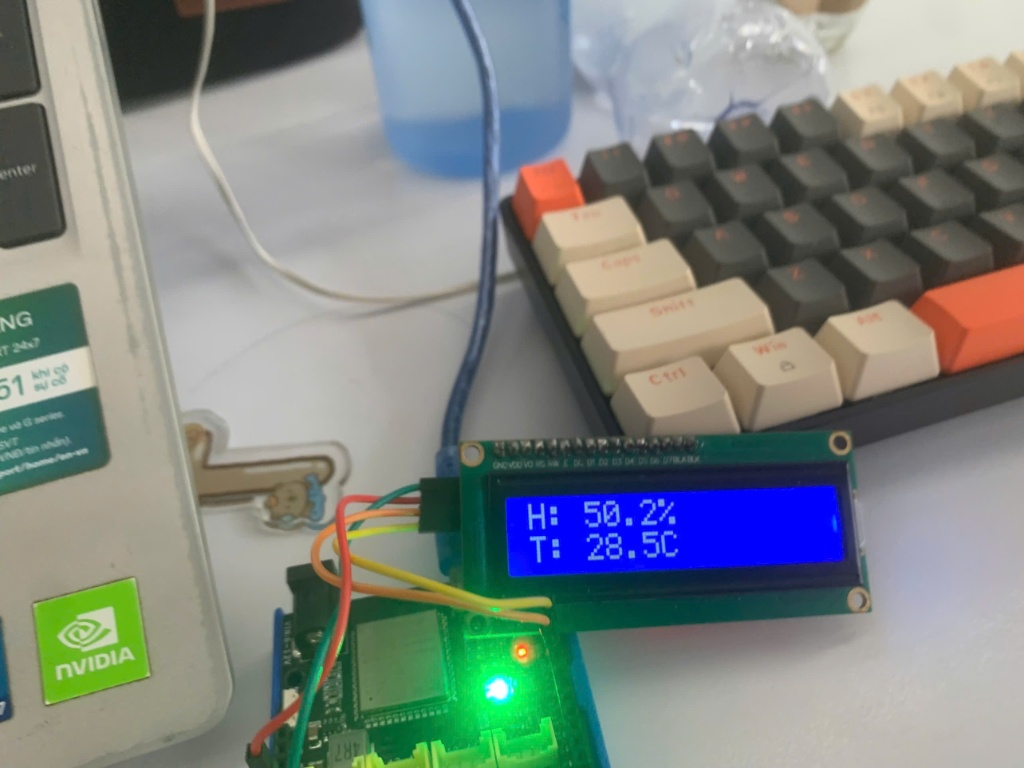
\includegraphics[width=0.75\linewidth]{picture/kq_task_12.png}
    \label{fig:placeholder}
\end{figure}

\begin{itemize}
    \item Led và NeoPixel phản hồi với nhiệt độ độ ẩm đọc từ cảm biến bằng màu sắc 

\end{itemize}

\subsubsection{Task 3: Giám sát môi trường qua LCD}

\begin{itemize}
    \item \textbf{Hiển thị thời gian thực:} Ở chế độ thông thường, màn hình cập nhật chính xác các thông số môi trường 
    \item \textbf{Cơ chế ngắt cảnh báo:} Khi xảy ra sự kiện quá nhiệt (28.4°C > 25°C), màn hình lập tức xóa dữ liệu cũ và thực hiện hiệu ứng chớp tắt dòng chữ \texttt{! WARNING TEMP !} ở hàng trên.
\end{itemize}

\subsubsection{Task 4: Máy chủ Web cục bộ (Local Web Server)}
\begin{figure}[H]
    \centering
    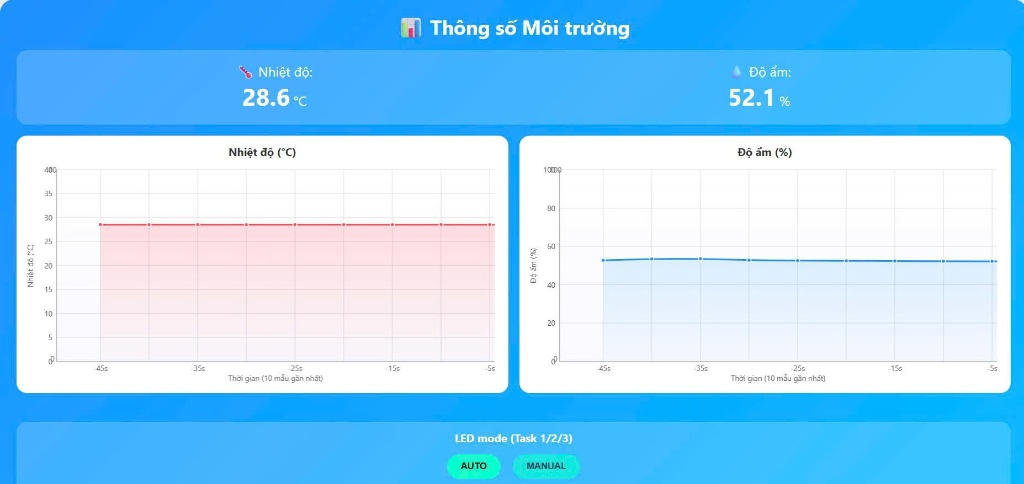
\includegraphics[width=0.75\linewidth]{picture/web_das.png}
    \label{fig:placeholder}
\end{figure}
\begin{figure}[H]
    \centering
    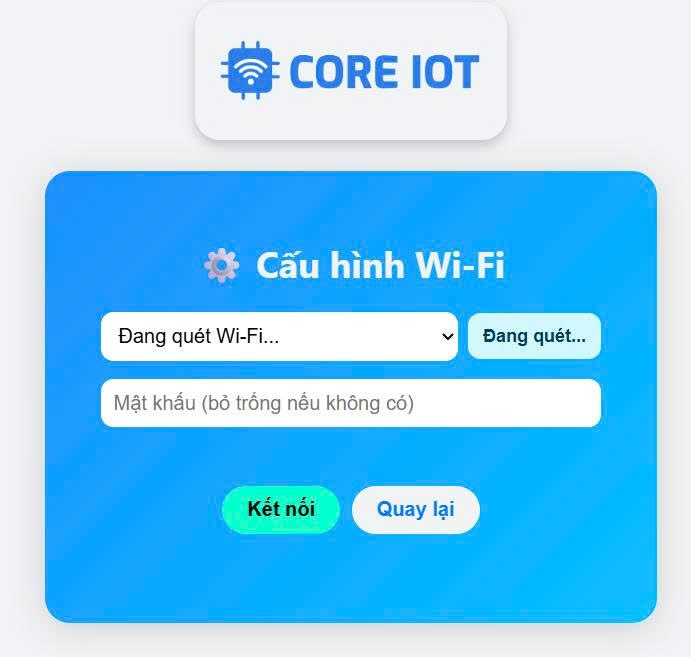
\includegraphics[width=0.75\linewidth]{picture/STA.png}
    \caption{Scan wifi kết nối sang chế độ STA}
    \label{fig:placeholder}
\end{figure}

\begin{figure}[H]
    \centering
    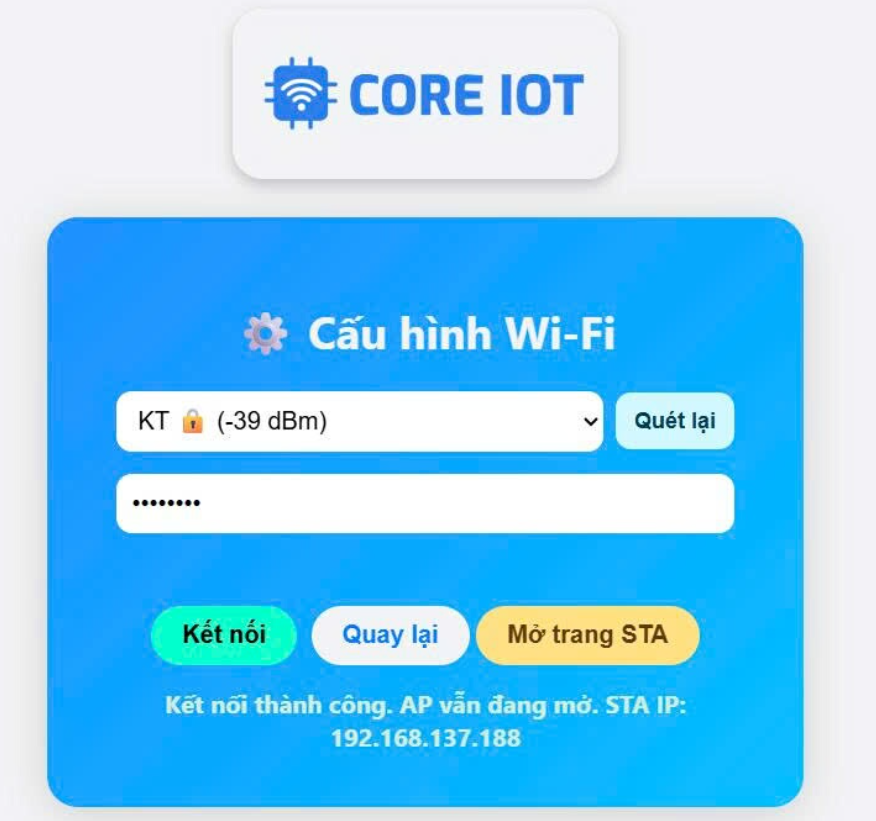
\includegraphics[width=0.6\linewidth]{picture/wifi_connect.png}
    \caption{Sau kết nối wifi thành công}
    \label{fig:placeholder}
\end{figure}

\begin{itemize}
    \item \textbf{Cấu hình mạng (AP Mode):} Cung cấp giao diện "Cấu hình Wi-Fi" , cho phép người dùng quét và nhập mật khẩu kết nối mạng nội bộ. Sau khi kết nối thành công với wifi sẽ cung một địa chỉ IP mới ở chế độ STA.
    \item \textbf{Giám sát nội bộ (SPA Dashboard):} Giao diện Web hiển thị số liệu trực quan với biểu đồ thời gian thực cho cả Nhiệt độ  và Độ ẩm. Các khối chức năng điều khiển chế độ LED (AUTO/MANUAL) và tinh chỉnh màu sắc đều hiển thị.
\end{itemize}

\subsubsection{Task 5: (TinyML)}
\begin{figure}[H]
    \centering
    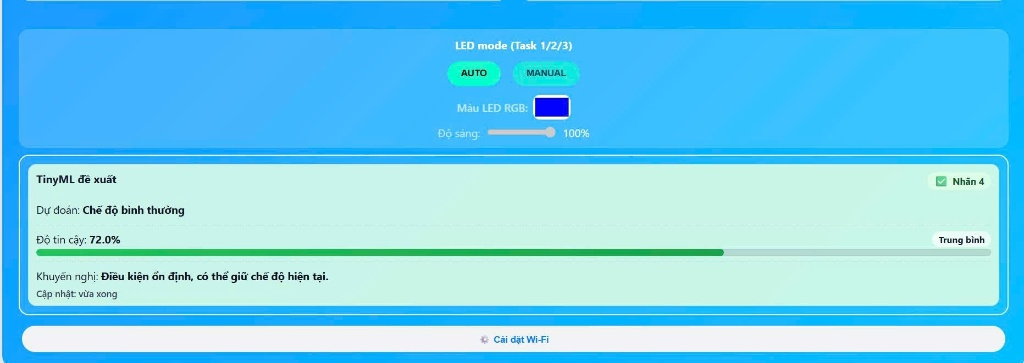
\includegraphics[width=0.75\linewidth]{picture/ml.png}
    \label{fig:placeholder}
\end{figure}




Thuật toán Naive Bayes được nhúng thành công và có khả năng đưa ra các suy diễn logic ngay trên phần cứng hạn chế của ESP32:
\begin{itemize}
    \item Thông qua giao diện Web, hệ thống trả về kết quả dự đoán "Chế độ bình thường" (Nhãn 4) với độ tin cậy (Confidence) đạt 72.0%.
    \item Dựa trên kết quả này, hệ thống chủ động đưa ra khuyến nghị: "Điều kiện ổn định, có thể giữ chế độ hiện tại". Điều này chứng minh tính thực tiễn của Edge AI trong việc hỗ trợ ra quyết định.
\end{itemize}

\subsubsection{Task 6: Tích hợp đám mây CoreIoT}
\begin{figure}[H]
    \centering
    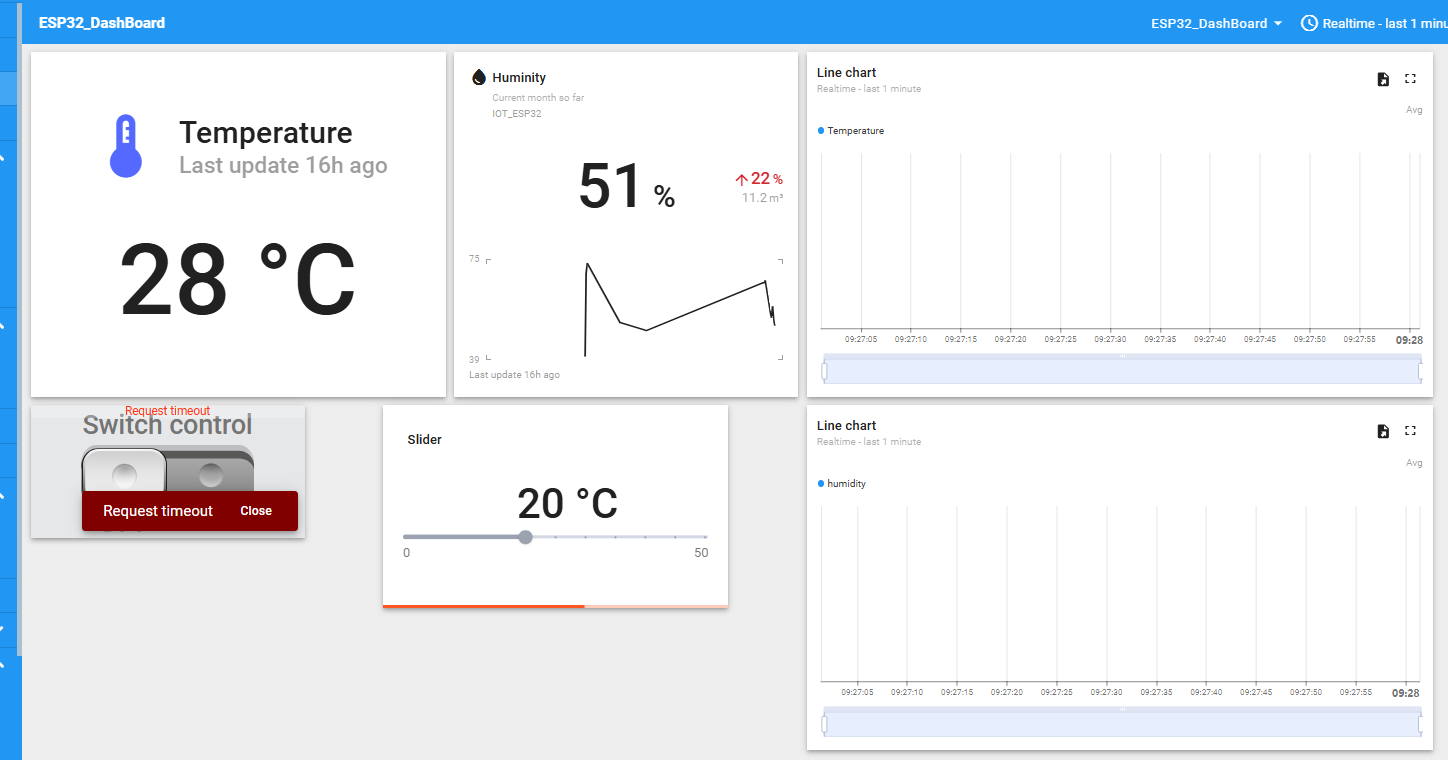
\includegraphics[width=0.75\linewidth]{picture/coreiot.png}
    \caption{Cấu hình ngưỡng nhiệt độ trên CoreIot}
    \label{fig:placeholder}
\end{figure}


\begin{figure}[H]
    \centering
    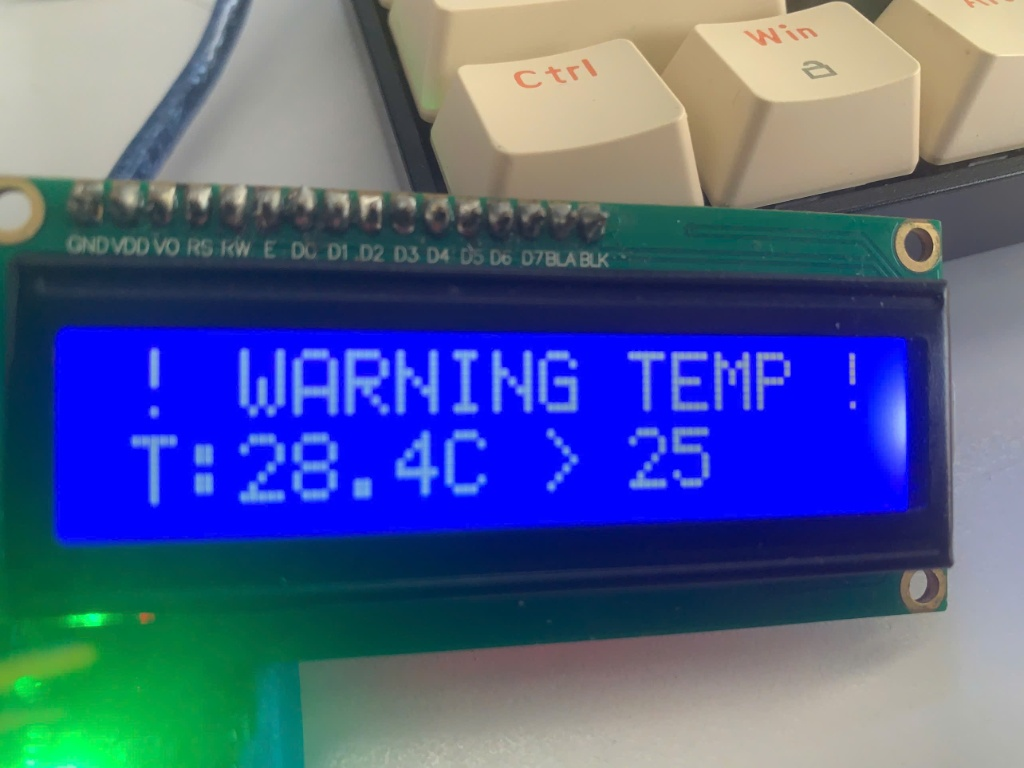
\includegraphics[width=0.75\linewidth]{picture/warning.png}
    \caption{Phản hồi thiết bị với ngưỡng nhiệt độ mới}
    \label{fig:placeholder}
\end{figure}


\begin{itemize}
    \item \textbf{Đồng bộ  (Telemetry):} Dashboard trên ThingsBoard nhận và trực quan hóa dữ liệu ổn định 
    \item \textbf{Điều khiển RPC và Xử lý ngoại lệ:} Thanh Slider thiết lập ngưỡng nhiệt độ (setThre) hoạt động  (ang ở mức 20°C.
\end{itemize}



\subsection{Tóm tắt chương}

Chương này đã trình bày các kết quả kiểm thử và đánh giá của hệ thống sau khi hoàn thiện. Ở phần kết quả chức năng, các chức năng chính của hệ thống đã được kiểm tra để xác nhận tính ổn định, khả năng hoạt động đúng theo yêu cầu và mức độ đáp ứng trong thực tế. Bên cạnh đó, phần đánh giá TinyML cho thấy mô hình có thể được triển khai hiệu quả trên thiết bị biên với tài nguyên hạn chế, đồng thời vẫn bảo đảm được sự cân bằng giữa độ chính xác, dung lượng bộ nhớ sử dụng và tốc độ suy luận. Từ các kết quả đạt được, có thể khẳng định giải pháp đề xuất phù hợp với định hướng ứng dụng IoT kết hợp AI nhúng và có tính khả thi khi triển khai thực tế.


